\section{Gamification}

When it comes to rehabilitation, consistent practice plays a crucial role. 
We know that gamification is key to enhancing patient engagement and consistency in practicing exercises.
By transforming repetitive tasks into enjoyable experiences, 
we aim to motivate patients and provide a more stimulating recovery process. 
This section details the software design, game adaptation and AI integration of gamified exercises.

\subsection{Requirements and Design Choices}
We have identified the following core requirements for the gamification software:
\begin{enumerate}
    \item \textbf{Engaging Gameplay}: Implement or adapt simple, intuitive game controls 
    that respond to varying pressure levels from the hand rehabilitation device,
    \item \textbf{Therapeutic Relevance}: UI and gameplay should be designed with therapeutic purposes in mind, 
    and be relevant to stroke rehabilitation (e.g., grasping, releasing, sustained pressure).
    \item \textbf{Visual Feedback}: Provide clear and immediate visual feedback corresponding to the patient's force input. 
    \item \textbf{Input Modality}: Support both single-input (1-Dome) and multi-input (3-Dome) device configurations.
    \item \textbf{User Interface}: Provide a clear interface for patients for selection, launching and for therapists to monitor measurements and analysis.
    \item \textbf{AI Analytics}: The system should be able to analyze the patient's performance and provide feedback to the therapist using AI.
    \item \textbf{Extensibility}: The system should be designed to easily incorporate new games and features in the future.
\end{enumerate}

Several key design choices were made to meet these requirements.

First of all, we have chosen web-based technology to develop the software, such as HTML, CSS and JavaScript. 
This enables us: (1) to develop the UI in a web browser, enabling cross-platform including mobile devices,
(2) to take advantage of visual design and user experience well-provided by the web technology stack, and
(3) to make use of the vast amount of existing open-source web-based games.

Second, we have chosen an event-driven architecture to handle inter-component communication.
By leveraging the existing event-driven mechanism of the web platform, we can easily decouple different components of the system.
This enables us to develop a modular design to allow for easy incorporation of new games and features in the future.

Third, we have experimented with different strategies to process force input from the device.
We used methods such as thresholding and direct mapping to map input to game actions.
Coupled with AI models that are able to analyze force input from the patient, 
we can provide feedback to the patient and potentially dynamically adjust the game parameters.

Fourth, we have adapted games to be more relevant to the rehabilitation process. 
Games are typically designed for entertainment and most require fast response time and challenging game controls. 
We selected games that are more relevant to force input(correspond to patient's hand movement) 
and adapted them to be more friendly to the patient(e.g. simplified controls, adjusted difficulty, etc.).

These choices aim to create a flexible, maintainable, and scalable gamification framework that can effectively support the rehabilitation process.


\subsection{User Interface Design}
The user interface provides users with intuitive access to the gamified rehabilitation exercises. 
The primary interaction points for gamification are located within the main panel of the application. 
The Gamified Exercises tab displays available games as a series of interactive "cards". 
\begin{figure} [h!]
    \centering
    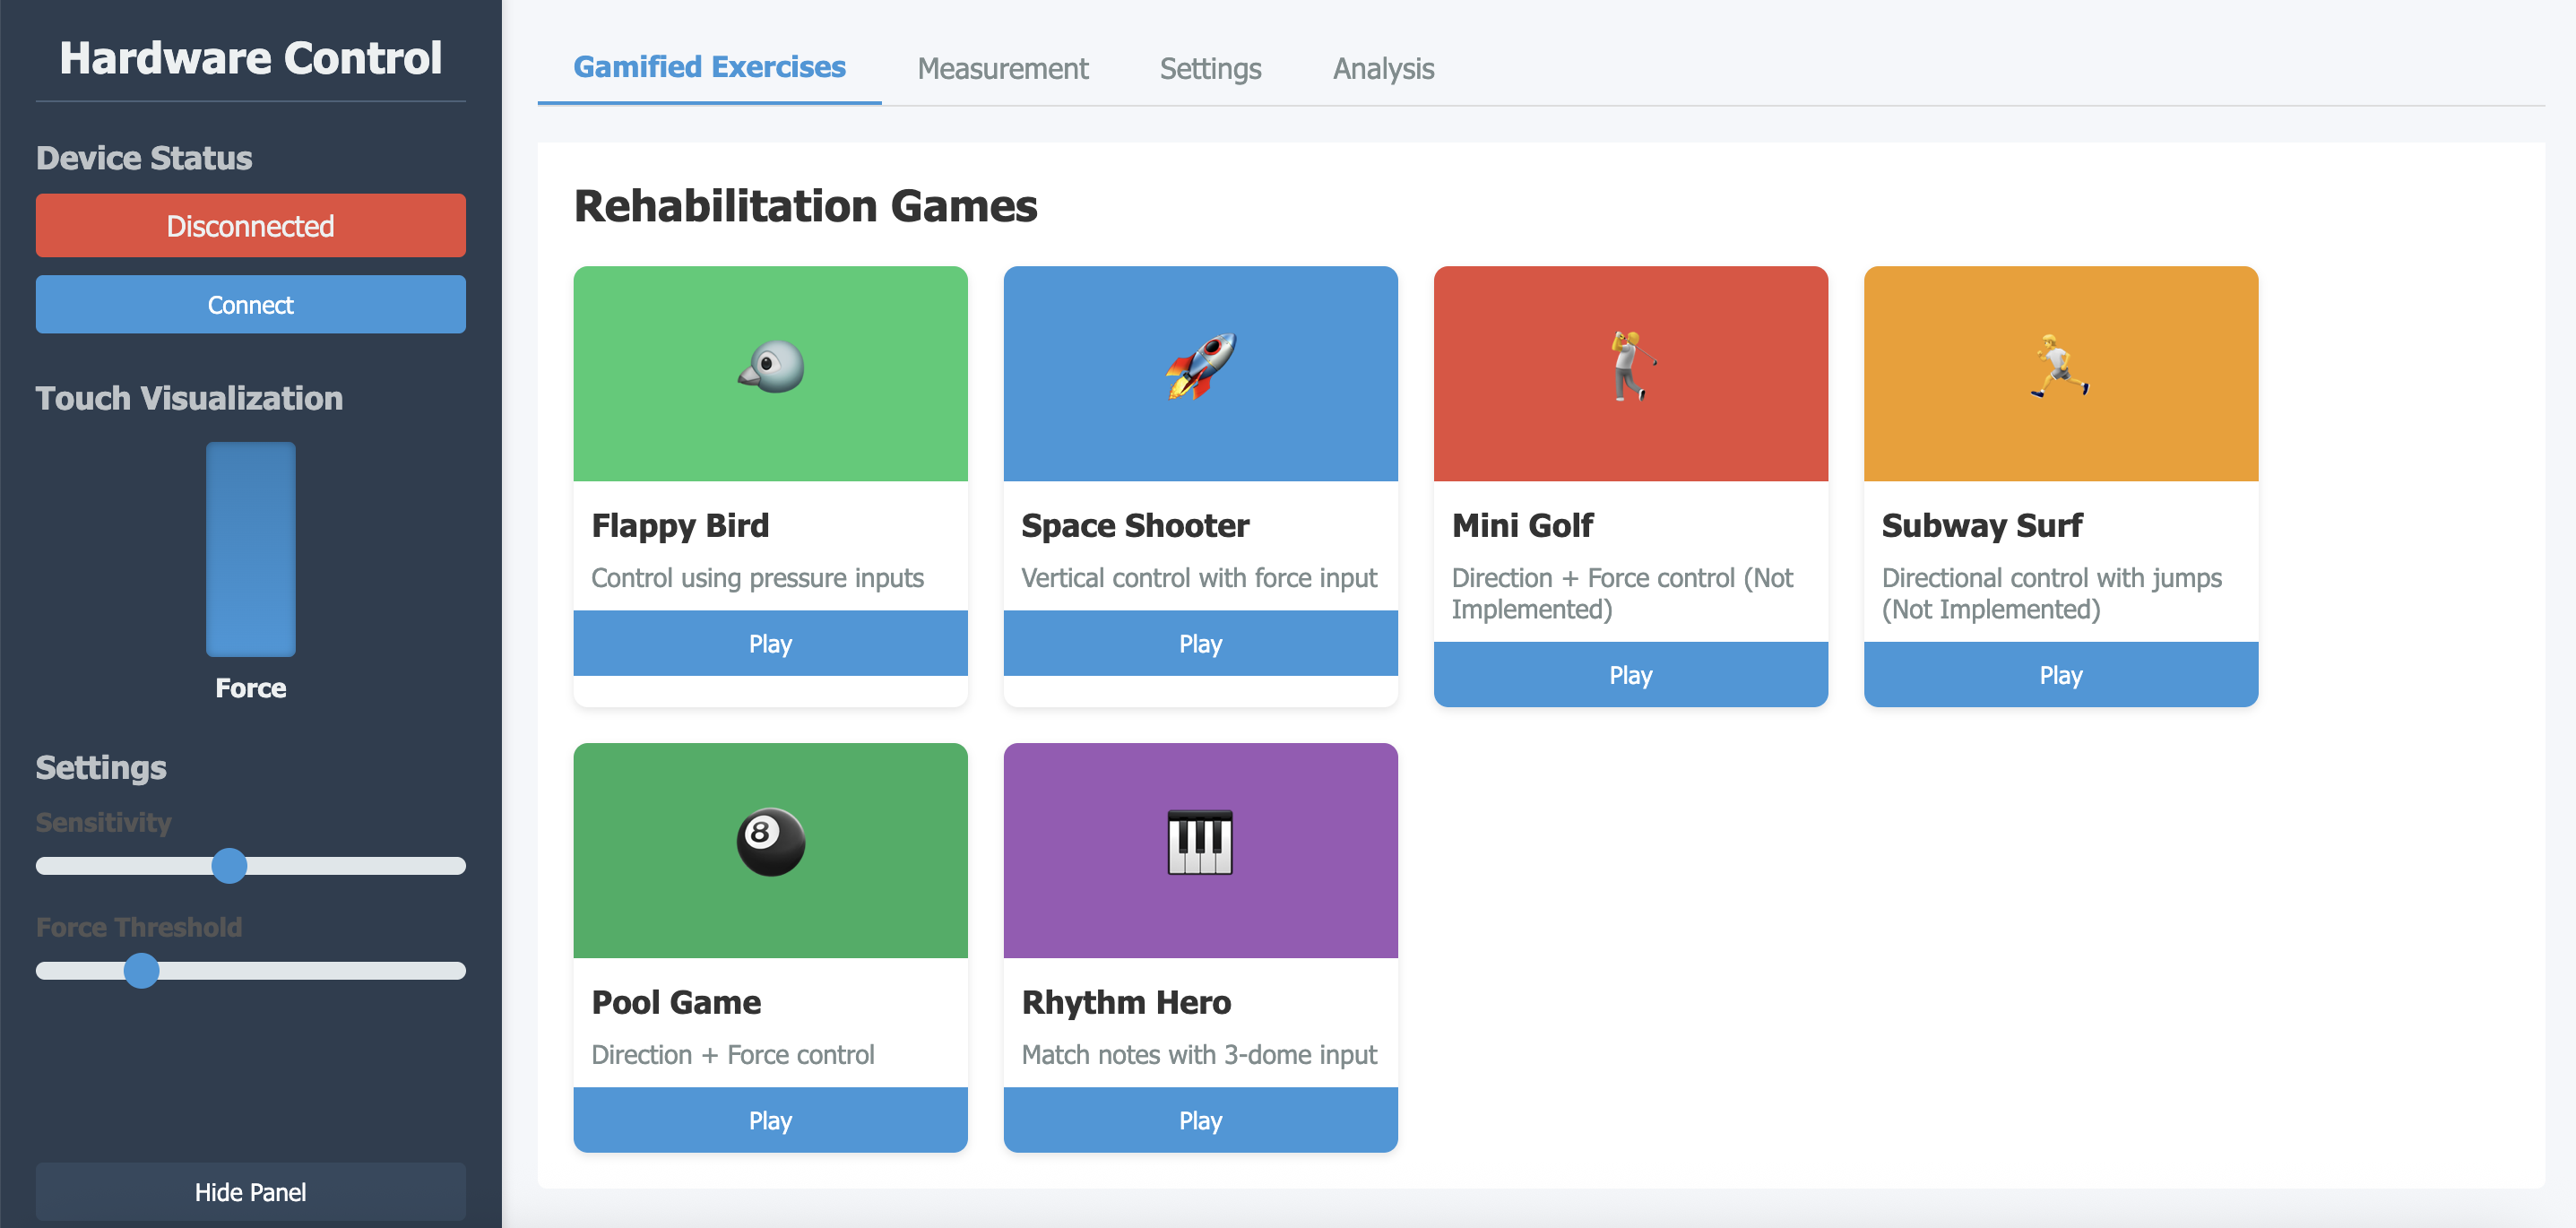
\includegraphics[width=0.8\linewidth]{Figures/ui_main.png}
    \caption{User Interface for Gamification}
    \label{fig:ui_main}
\end{figure}

When a game is launched, its specific interface is displayed within a dedicated area in the main panel. 
Then game logic takes over and the user can interact with the game. 
\begin{figure} [h!]
    \centering
    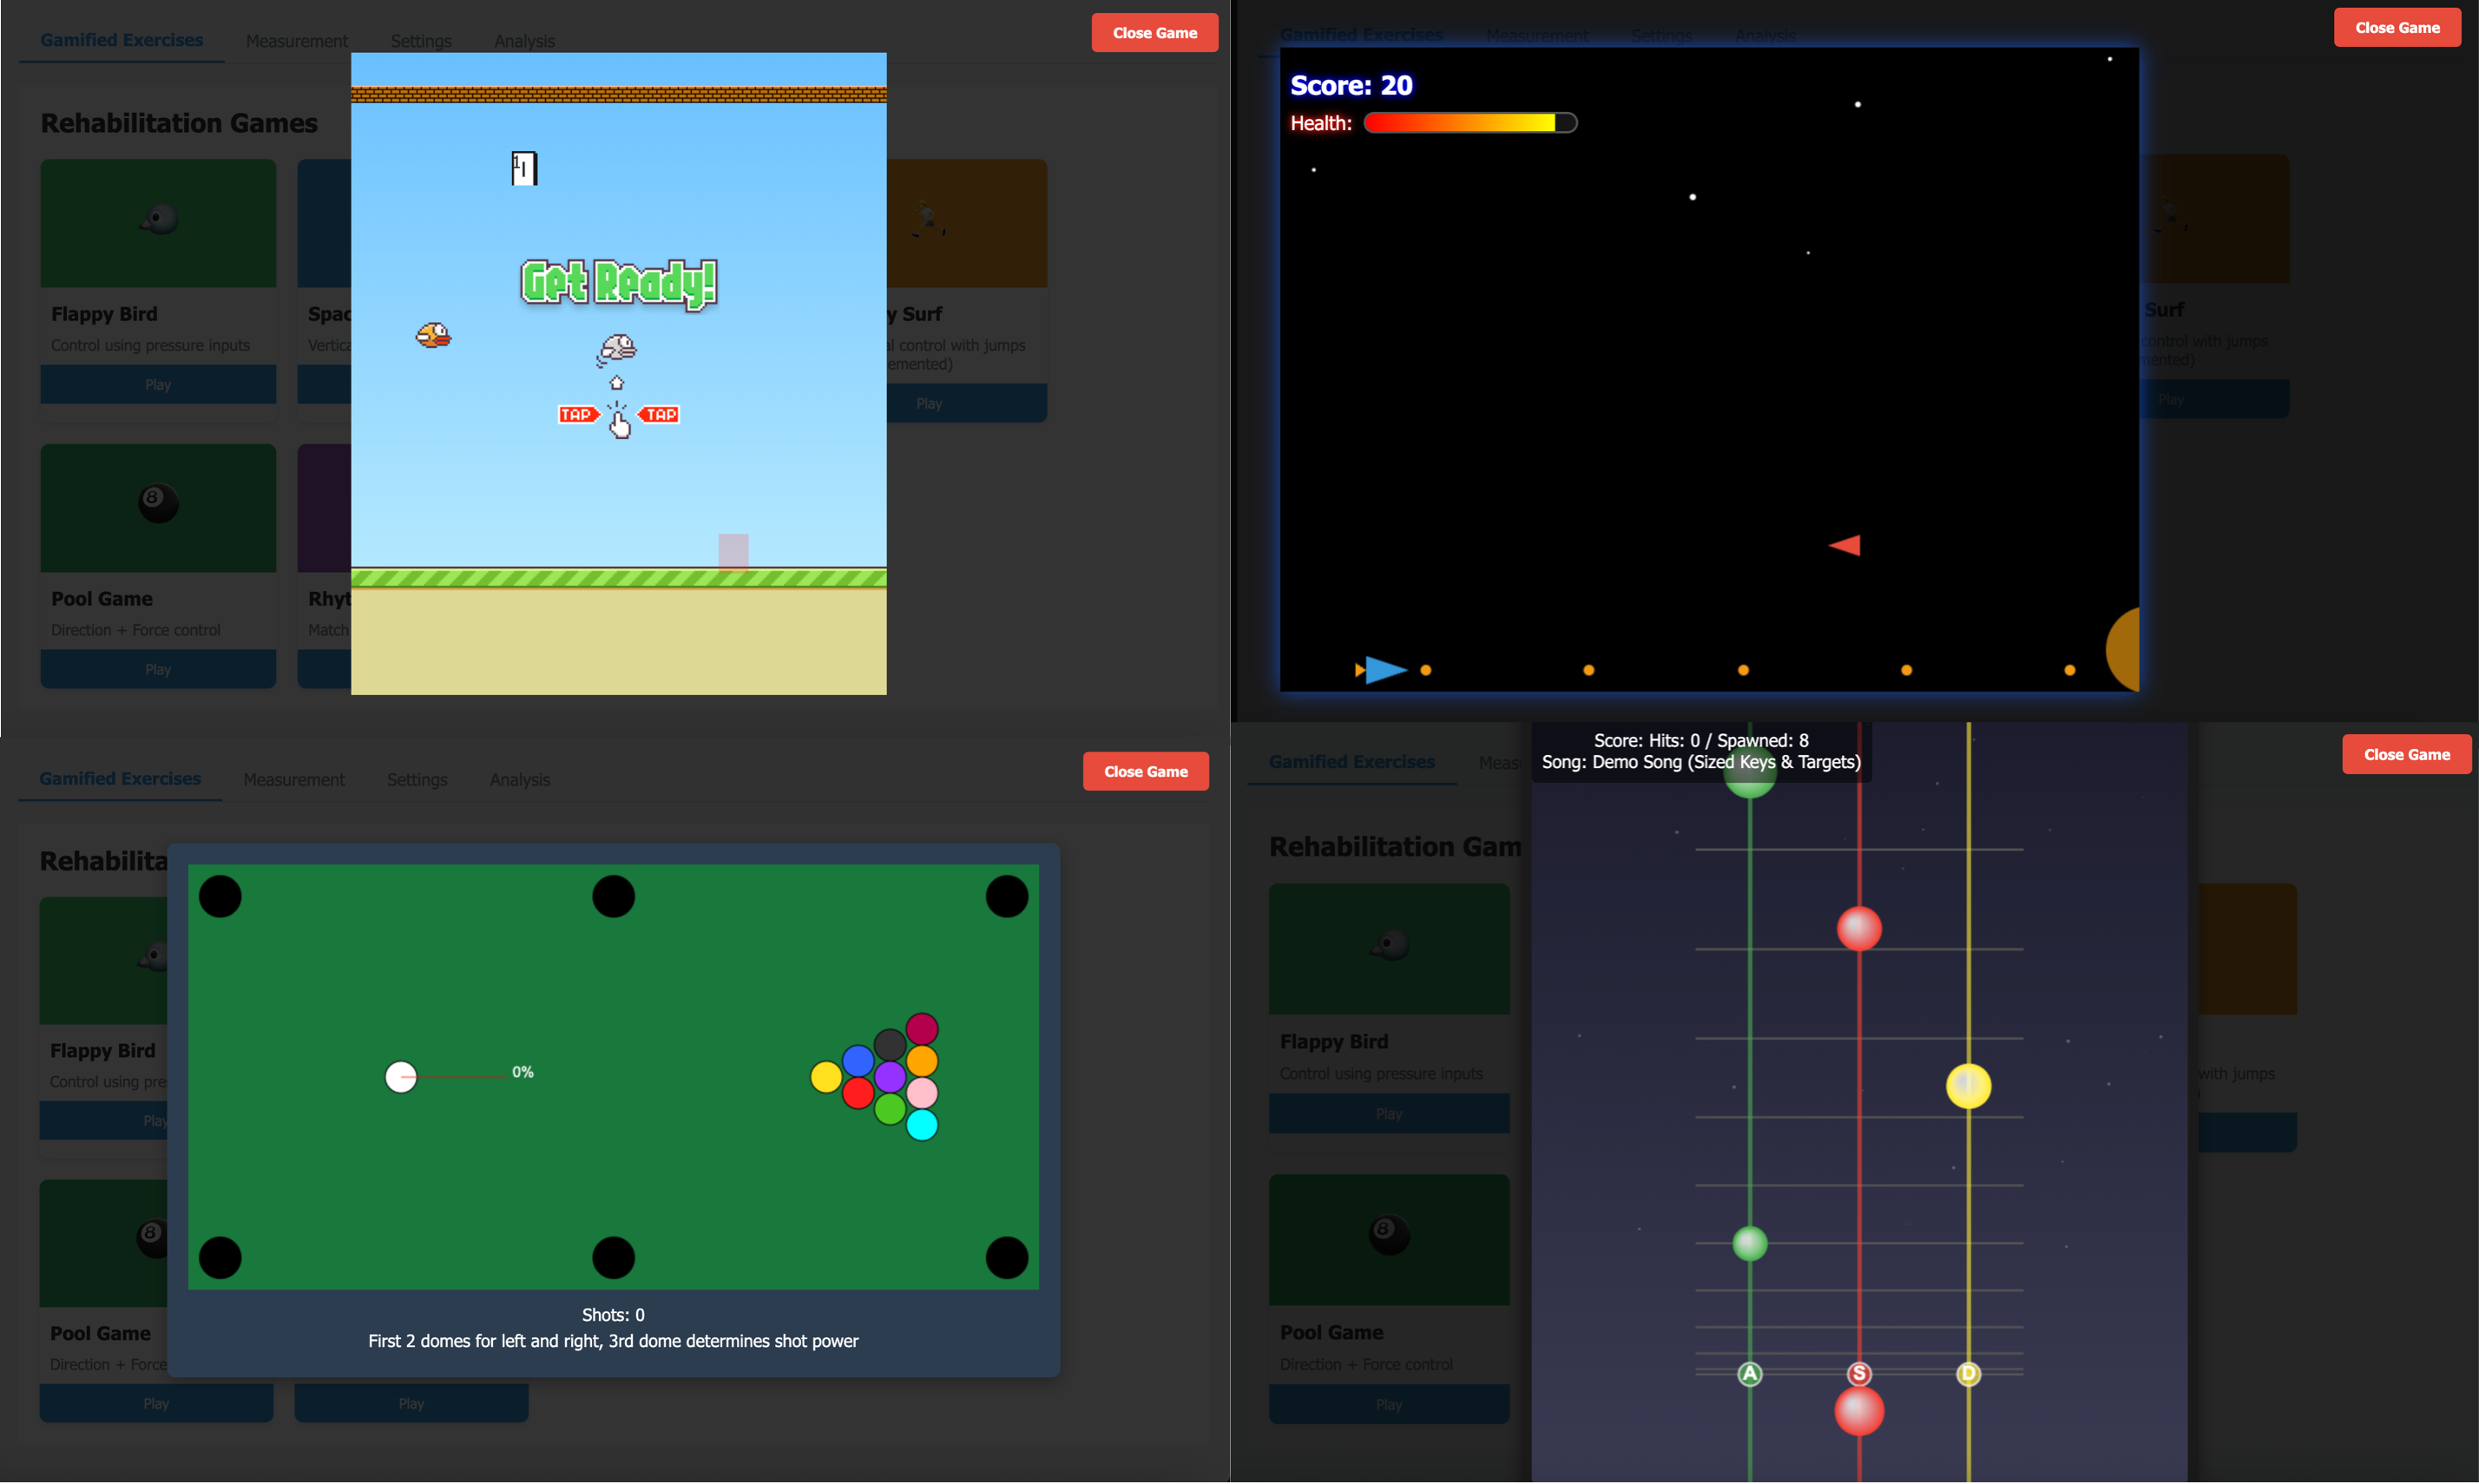
\includegraphics[width=0.8\linewidth]{Figures/ui_games.png}
    \caption{Already adapted games, namely Flappy Bird, Space Shooter, Pool Game and Rhythm Hero.}
    \label{fig:ui_games}
\end{figure}

There are 3 other tabs in the main panel, namely:
\begin{itemize}
    \item \textbf{Measurements}: Users can monitor the measurements from the device.
    \item \textbf{Settings}: Hardware settings, device calibration, simulation control etc.
    \item \textbf{Analysis}: AI model analysis and feedback.
\end{itemize}

The left side panel provides a quick overview of the current device status, force bars visualization and shortcuts. 
It can be hidden.

The overall UI design aims for clarity and ease of use, with minimal steps to engage with the therapeutic games. 

\subsection{Software Design}
The system employs an event-driven architecture centered around an \texttt{InputModeManager} 
that handles data acquisition from either a physical device (via Web Serial API) or a simulator. 
Force data is processed, normalized, and then broadcasted via a global \texttt{EVT\_FORCE\_UPDATE} event.

A \texttt{game\_control} module acts as the central coordinator for games control. 
It listens for \texttt{EVT\_FORCE\_UPDATE} events and, based on the currently active game, 
directs the force data to the respective game's input handling functions. 
Each game is encapsulated within its own script (e.g., \texttt{flappybird.js}, \texttt{spaceshooter.js}, \texttt{poolgame.js}, \texttt{rhythmkeys.js}), 
responsible for its own game logic, rendering, and state management. 
These game scripts expose apis to the \texttt{game\_control} module.

This decoupled design offers several advantages:
(1) Individual games can be developed, tested, and updated independently.
(2) New games can be added with minimal changes to the core input handling system.
(3) Boundaries between the input system, game controller, 
and individual games simplify debugging and development.
(4) Simulation mode is supported to allow for testing and debugging without the need of a physical device.

UML diagrams illustrating this architecture can be found in Appendix Fig.~\ref{fig:software_arch}.

As for the data flow(sequence diagram can be found in Appendix Fig.~\ref{fig:software_sequence}), in \texttt{simulation} mode, the \texttt{InputModeManager} uses a \texttt{SimulatedSerialPort} that can generate data based on keyboard inputs (Spacebar for 1-dome, A/S/D for 3-dome).
 In \texttt{arduino} mode, it uses \texttt{ArduinoConnection} to interface with the physical device via the Web Serial API.
Regardless of the source, raw pressure data is normalized into a 0-1 range(max range is set by calibration).
The \texttt{InputModeManager} then dispatches an \texttt{EVT\_FORCE\_UPDATE} custom event, including the normalized force, raw pressure and device type.

During the game, force data is processed by individual game scripts 
and transmiited to AI analysis server after one session is finished(partially implemented).
Then the AI analysis server will provide feedback to the user via the Analysis tab.

\subsection{Game Adaptation}
We have adapted four games to be more relevant to the rehabilitation process. 
The original game implementations are from open-source projects on Github.
They are selected because they are simple and intuitive and a connection with force input is apporiate.
The adaptation is done by modifying the game logic to be more relevant to the rehabilitation process.

\subsubsection{Flappy Bird}
This game controls a bird to flap and navigate through pipes. The original game control is too fast and easily failing. 
Therefore, the difficulty was adjusted to more friendly(two pipes to 1 pipe, reduced speed, lower gravity, etc.).
It is connected to the force input by using a simple threshold, i.e. when the force input exceeds a predefined threshold, the bird will flap.
This could be connected to grasp and release patterns of the hand, especially pinching movement.

\subsubsection{Space Shooter}
This game controls a ship to move vertically, shooting incoming enemies. It was adjusted to limit the ship's movement to up and down.
The force input linearly maps to the ship's vertical position. This allows analog control of the ship's movement, 
in contrast to the discrete control in Flappy Bird case. It requires a finer control of dome pressure, 
which could be useful for the advanced stage of rehabilitation process.


\subsubsection{Pool Game}
This simple game controls a cue stick to hit pool balls. The game is to be played with 3-dome device. 
The first 2 force inputs control the left and right movement of the cue stick using thresholding, while 
the third force input is mapped to the shot power. This combination of control mechanism shows the potential of
different possible configurations of the device for different rehabilitation exercises. 
For example, the first 2 force inputs may come from the thumb and index finger, while the third force input may come from the general gripping.

\subsubsection{Rhythm Hero}
This game is a rhythm game, where notes fall in multiple lanes. The player must hit corresponding lanes as notes reach a target zone, with background music.
It is controlled by the 3-dome device. Each force input is connected to the note hitting of each lane by using dynamic thresholds. 
For now, random thresholds are set by the game logic and appear as bigger or smaller notes. This introduces more rhythm to the exercise.
Potentially, we can leverage AI models to dynamically adjust the thresholds based on the patient's performance. 

Different adaption strategies were experimented. Game logic and difficulty should be adjusted to be more friendly to the rehabilitation process. 
A key design choice is how force input is used for game control. We implemented different strategies, 
such as thresholding(discrete), direct mapping(analog), mixed(discrete and analog), and dynamic thresholds, etc. 
Together with configurability of the device, it shows the potential of accomodating to different rehabilitation exercises.


\subsection{AI Integration}




\subsection{Future Considerations}

Future work includes:

Dynamic Difficulty Adjustment:
The game parameters such as difficulty, duration, etc. could be adjusted dynamically. 
We want to make the game playful for different stages of the rehabilitation process,
which means the difficulty level should be accomodating to the patient's current ability.
Another challenge is to balance the playfulness and the patient's exercise intensity.

Configurability:
For now, the device has two configurations, 1-dome and 3-dome. 
Future software should support different configurations in a flexible way.

Advanced Signal Processing
The pressure measurement can be affected by temperature and other environmental factors. 
Since environmental dynamics are slower than pressing dynamics, we could use 
the higher frequency component of the pressure signal for game control and analysis.








